\documentclass[conference]{IEEEtran}
\hyphenation{op-tical net-works semi-conduc-tor}
\usepackage{amsthm,amssymb,amsmath}
\usepackage{algorithmic}
\usepackage{graphicx}
\usepackage{bm}
\usepackage{array}
\usepackage{cite}
\usepackage{url}
\usepackage{gensymb}
\usepackage[justification=centering]{caption}

\begin{document}

\title{An Open Source Covariate based Software Reliability Assessment Tool}

\author{\IEEEauthorblockN{Author1 Name$^1$, Author2 Name$^1$, and Lance Fiondella$^1$}
\IEEEauthorblockA{$^1$Electrical and Computer Engineering, University of Massachusetts Dartmouth, MA, USA\\
	%}
%\IEEEauthorblockA{$^2$Naval Air Systems Command, Patuxent River, MD, USA\\
Email: \{lfiondella\}@umassd.edu}
}
%\and
%\IEEEauthorblockN{Thierry Wandji}
%\IEEEauthorblockA{Naval Air Systems Command}
%	Email: }
%Telephone: }

\maketitle

\begin{abstract}%Need to be revised
This paper presents an open source covariate based software reliability tool to automatically apply methods from software reliability engineering to incorporate covariate data to enable inferences about the software testing process. The tool provides functionalities including visualization of failure data, application of software reliability growth models including various hazard rate funtions, inferences made possible by these models, and assessment of goodness of fit. The application and source code are available through the web. The open source nature of this tool will enable unprecedented levels of collaboration among researchers and practitioners from industry and government within a single shared platform.
\end{abstract}

\begin{IEEEkeywords}
Software reliability, software reliability growth model, covariates, Python programming language, GitHub
\end{IEEEkeywords}


\section{Software Reliability Engineering}
What is NHPP SRGM? Why Covariate NHPP SRGM?

Existing tools. Reason for developing this tool.

Contribution.


Section~\ref{sec:SRAT} provides a brief overview of the tool's user interface, which is divided into three primary activities, including selection, analysis, and filtering Data~\ref{sec:Tab1}, model fit and prediction ~\ref{sec:Tab2}, and model evaluation~\ref{sec:Tab3}. Section~\ref{sec:Concl} concludes the paper and identifies future work.

\section{Covariate based Software Reliability Assessment Tool (CSRAT)}\label{sec:SRAT}
This section presents detailed discussion of the functionalities implemented in the tool and how to use it.

\subsection{Tab1: }\label{sec:Tab1}
Figure \ref{} shows.....Add more
\\
\\
Users can begin using the tool by uploading a data file in either an Excel spreadsheet (.xlsx) or a CSV file (.csv). The first column in the input file will be used as failure time data (FT), the second column as number of failures with respect to time, and subsequent columns as covariate data sets. The header names will not effect how the data is treated other then the covariate data names displayed in the \textbf{Select Metric(s)} box found as figure \ref{} shows. If header names are not given, by default the program will label the missing covariate items "Metric\textit{n}" with \textit{n} being the position in the list.

%Second tab for the tab with the covariate selection box

The user can upload a new file by rolling over the \textbf{File} option in the system menu and clicking on \textbf{Open} in the drop down menu. The upload is successful, when the "MVF" (mean value function) plot and data are populated. Figure \ref{} shows the large box which shows the plot or table, toggled by \textbf{Plot} and \textbf{Table} tabs. The \textbf{Metric(s)} box will also show a list of the available covariate data found in the file.

For the top of the left column shown in Figure \ref{fig:tab1_left_column}, users will find the \textbf{Select Sheet} pull down menu. If more than one sheet exisits in the data file, the user can specify which sheet to display and use. 

The following two boxes labeled \textbf{Select Model(s)} and \textbf{Select Metric(s)}, include the selections for the hazard function models and covariate data sets. In both boxes, users can select one or more of each option by clicking on a label which will highlight it. Clicking on a the label again will deselect the option. Additionally, users can hold click and drag over a list region to toggle all options within the region.

\begin{figure}[!ht]
	\centerline{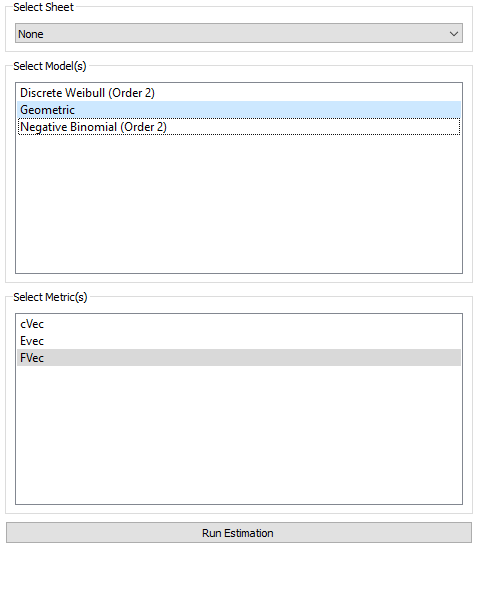
\includegraphics[width=\columnwidth]{Figures/tab1_left_column.PNG}{}}
	\caption{Tab 1 Left Column}
	\label{fig:tab1_left_column}
\end{figure}

%\begin{figure}[!h]
%\centering
%\includegraphics[width=3.5in]{Figures/FigureName}
%\caption{Tab one options}
%\label{fig:xxx}
%\end{figure}


\subsection{Tab2: }\label{sec:Tab2}
Description

Figure 

\subsection{Tab3: }\label{sec:Tab3}
Description

Figure 

\section{Conclusion and Future Research}\label{sec:Concl}
This paper presents an open source...

\section*{Acknowledgment}
This material is based upon work supported by the National Science Foundation under Grant Number (\#1749635). Any opinions, findings, and conclusions or recommendations expressed in this material are those of the authors and do not necessarily reflect the views of the National Science Foundation.

\bibliographystyle{IEEEtran}
\bibliography{bibIEEE}


\end{document}


